\documentclass{article}
\usepackage{ctex}
\usepackage{graphicx}
\usepackage{amsmath}
\usepackage{amssymb}
\usepackage{hyperref}
\usepackage{subcaption}

\title{HW01-1 FNN 超参数实验报告}
\author{姓名: 刘行\\学号: PB22000150}
\date{\today}

\begin{document}
\maketitle
	\section{引言}
		本实验旨在研究不同超参数设置对前馈神经网络 (FNN) 在波士顿房价数据集上的表现. 通过调整网络深度, 学习率和激活函数, 我们分析它们对模型训练损失和验证损失的影响.

	\section{代码思路}
		本代码实现了一个前馈神经网络 (FNN) 用于回归任务, 并包含以下主要步骤:

		\begin{enumerate}
			\item \textbf{数据加载与预处理}: 使用\texttt{fetch\_openml}函数加载波士顿房价数据集, 并进行标准化处理, 以提高训练稳定性.
			\item \textbf{数据集划分}: 将数据集划分为训练集, 验证集和测试集, 分别用于模型训练, 超参数调优和最终评估.
			\item \textbf{模型定义}: 构建一个可配置的前馈神经网络, 允许用户调整隐藏层数目, 每层神经元数量及激活函数.
			\item \textbf{训练过程}: 使用均方误差 (MSE) 作为损失函数, 并采用 Adam 优化器进行梯度更新. 模型训练过程中, 每个 epoch 计算训练集损失和验证集损失.
			\item \textbf{超参数实验}: 对比不同的网络深度, 学习率和激活函数对模型性能的影响, 并绘制验证损失曲线进行分析.
			\item \textbf{最终模型评估}: 使用最优超参数重新训练模型, 并在测试集上计算最终损失.
		\end{enumerate}

	\section{实验设置}
		\begin{enumerate}
			\item \textbf{网络结构: }实验中我们选择了以下三种不同的网络深度进行对比:

				\begin{itemize}
					\item 单隐藏层: $\{32\}$
					\item 双隐藏层: $\{64, 32\}$
					\item 三隐藏层: $\{128, 64, 32\}$
				\end{itemize}

			\item \textbf{学习率: }我们选取了以下三种不同的学习率 $0.01, 0.001, 0.0001$ 进行实验

			\item \textbf{激活函数: }我们选择了 ReLU, Sigmoid 和 Tanh 作为隐藏层的激活函数, 并在相同的网络结构下进行实验对比.
		\end{enumerate}

	\section{实验结果}
		以特征字段 ``CRIM'' 为例, 实验结果如下图, 横坐标为轮次, 纵坐标为验证数据集的误差:

		\begin{figure}[htbp]
			\centering
			\begin{subfigure}[b]{0.45\textwidth}
				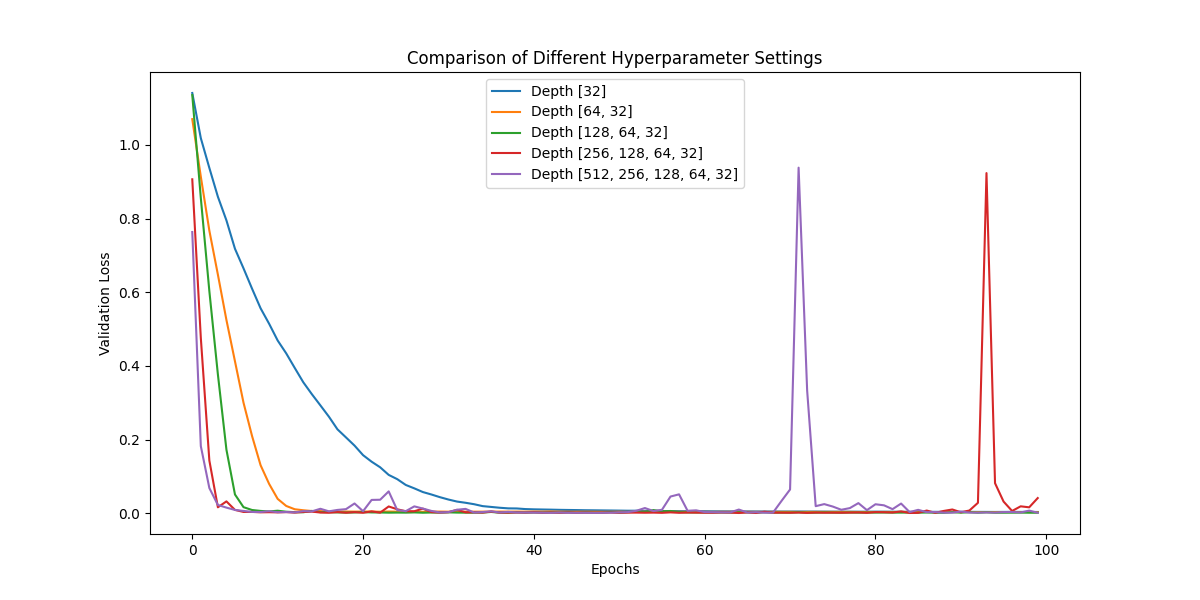
\includegraphics[width=\textwidth]{figure/depths.png}
				\caption{不同深度的比较}
			\end{subfigure}
			\begin{subfigure}[b]{0.45\textwidth}
				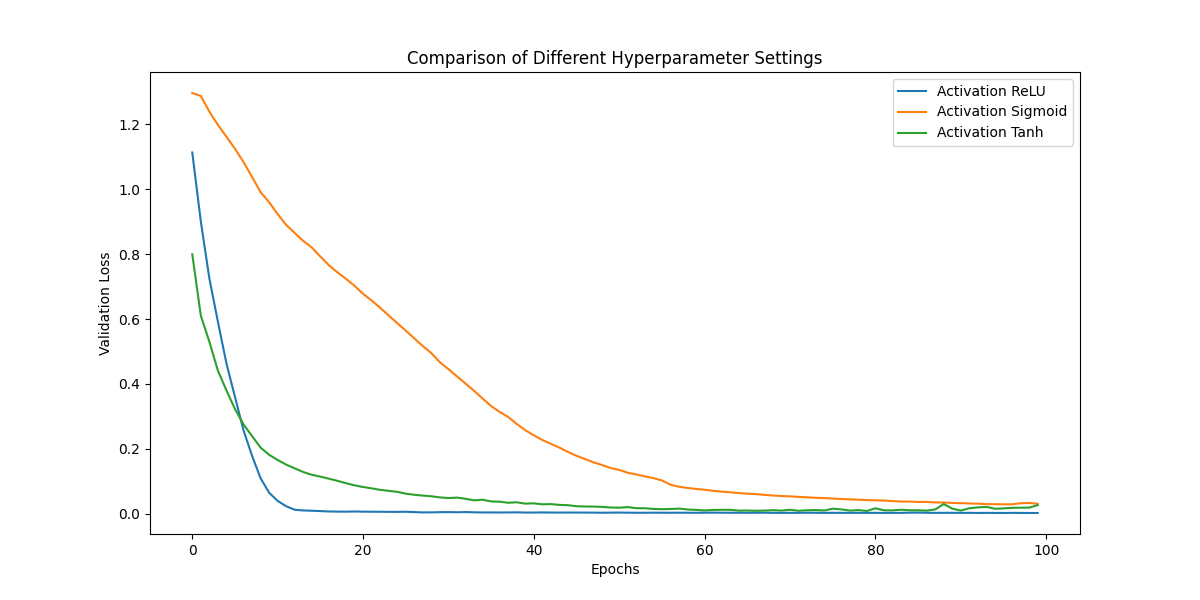
\includegraphics[width=\textwidth]{figure/activation_functions.png}
				\caption{不同激活函数的比较}
			\end{subfigure}
			\begin{subfigure}[b]{0.45\textwidth}
				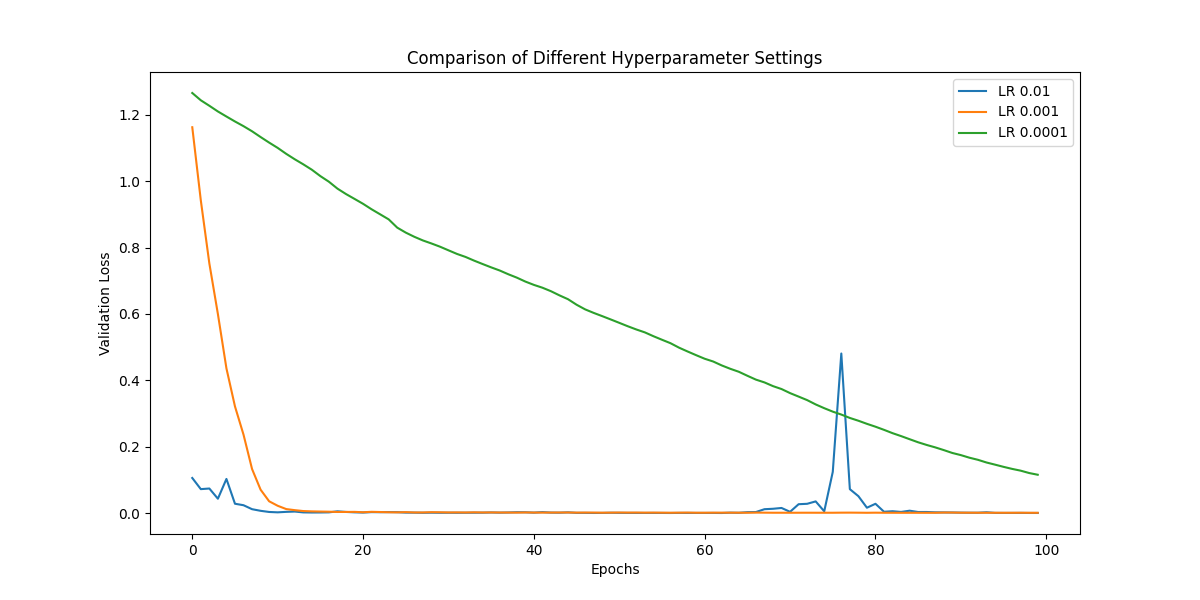
\includegraphics[width=\textwidth]{figure/learning_rates.png}
				\caption{不同学习率的比较}
			\end{subfigure}
			\begin{subfigure}[b]{0.45\textwidth}
				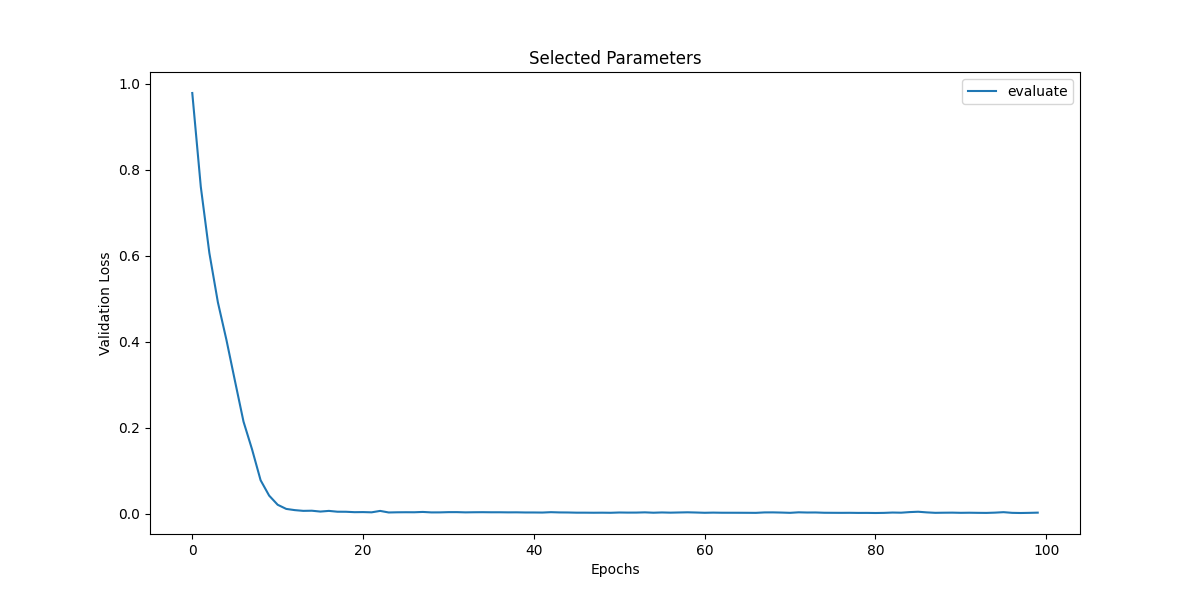
\includegraphics[width=\textwidth]{figure/selected_parameters.png}
				\caption{最终选定的参数}
			\end{subfigure}
		\end{figure}

		其中, 最终选定的参数分别为 2 层, ReLU, 0.001. 观察图像可得:

		\begin{itemize}
			\item ReLU 激活函数在本任务中表现优于 Sigmoid 和 Tanh, 因为其能够有效缓解梯度消失问题.
			\item 增加网络深度通常能够提高模型的学习能力, 但过深的网络可能会导致过拟合.
			\item 适中的学习率 (如 0.001) 在本实验中表现最佳, 学习率过大会导致模型难以收敛, 而过小的学习率则训练缓慢.
		\end{itemize}

	\section{代码亮点}
		本实验代码的主要亮点如下:

		\begin{enumerate}
			\item \textbf{模块化设计}:
				\begin{itemize}
					\item 代码采用面向对象的方式, 封装了 FNN 模型, 使得超参数调整更加灵活.
					\item 训练函数与超参数实验函数分离, 提高代码的可复用性.
				\end{itemize}
			\item \textbf{超参数实验对比}:
				\begin{itemize}
					\item 通过系统性实验对比不同超参数设置, 提高了实验的科学性.
					\item 使用 Matplotlib 绘制训练损失曲线, 直观展示不同超参数对模型性能的影响.
				\end{itemize}
			\item \textbf{自动数据预处理}:
				\begin{itemize}
					\item 采用标准化方法处理数据, 提高模型的收敛速度和稳定性.
				\end{itemize}
		\end{enumerate}

	\section{结论}
		本实验通过对比不同超参数设置, 得出以下结论:

		\begin{itemize}
			\item 在本数据集上, 深度适中的网络 (如 \{64, 32\}) 能够较好地学习数据特征.
			\item 选择适当的学习率 (如 0.001) 可以加速模型收敛, 同时避免梯度爆炸或梯度消失问题.
			\item ReLU 激活函数在本实验中表现最佳.
		\end{itemize}

		未来的研究可以进一步探索其他正则化方法 (如 Dropout) 或优化算法 (如 SGD) 对模型性能的影响.

\end{document}
